\section{TWSVM}

TWSVM (孪生支持向量机) 是 Jayadeva 等人于2007年提出的一种改进的双分界面支持向量机,用于解决二分类问题。与传统的支持向量机 (SVM) 不同,TWSVM 为每一类的数据点单独建立一个分类面,其优化策略为,使同一类的数据点尽可能集中的围绕在该类分类面的周围,并且远离另一类数据的分类面。所以 TWSVM 需要解决两个二次规划问题,得到两个不平行的分类面,但是同一类的数据要作为另一个二次规划问题的约束条件,反之亦然。

TWSVM 需要求解以下两个二次优化问题:
\begin{align}
\begin{split}
\label{ts1}
\min_{\mathbf{w}_1,b_1} \; & \frac{1}{2}\|\mathbf{Aw}_1+\mathbf{e}_1b_1\|_2^2+c_1\mathbf{e}_2^T\mathbf{q}_1 \\
s.t.\; & -(\mathbf{Bw}_1+\mathbf{e}_2b_1)+\mathbf{q}_1 \geq \mathbf{e}_2,\mathbf{q}_1\geq 0
\end{split}
\\
\begin{split}
\label{ts2}
\min_{\mathbf{w}_2,b_2} \; & \frac{1}{2}\|\mathbf{Bw}_2+\mathbf{e}_2b_2\|_2^2+c_2\mathbf{e}_1^T\mathbf{q}_2 \\
s.t. \; & (\mathbf{Aw}_2+\mathbf{e}_1b_2)+\mathbf{q}_2\geq \mathbf{e}_1, \mathbf{q}_2\geq 0
\end{split}
\end{align}
其中,$\mathbf{A}_{m_1 \times n}=(\mathbf{a}_1^{(1)},\mathbf{a}_2^{(1)},\ldots,\mathbf{a}_{m_1}^{(1)})^T$ 表示 $m_1$ 个正样本,$\mathbf{B}_{m_2 \times n }=(\mathbf{b}_1^{(2)},\mathbf{a}_2^{(2)},\ldots,\mathbf{a}_{m_2}^{(2)})^T$ 表示 $m_2$ 个负样本,$\mathbf{e}_1$ 和 $\mathbf{e}_2$ 表示相应维数的单位变量,$||\cdot||_2$ 表示L2范数,$\mathbf{q}_1, \, \mathbf{q}_2$ 是松弛向量,$c_1, \, c_2$ 是非负惩罚系数,分别为正样本和负样本的平衡因子,可以用来解决正负样本个数不同的问题。通过求解以上两个优化问题,可以分别得到两个不平行的超平面:
\begin{equation}
\mathbf{x}^T\mathbf{w}_1+b_1=0, \quad \mathbf{x}^T\mathbf{w}_2+b_2=0
\end{equation}
当有一个新的点 $\mathbf{x}$,计算其到两个超平面的垂直距离,如果它距离超平面 $\mathbf{x}^T\mathbf{w}_1+b_1=0$ 的距离小于它到超平面 $\mathbf{x}^T\mathbf{w}_2+b_2=0$ 的距离,则将该点归入正类,否则它属于负类。

我们也可以得到问题 \ref{ts1}、\ref{ts2} 的 Wolfe 对偶问题:
\begin{align}
\begin{split}
\max\limits_{\pmb{\alpha}} \; & \mathbf{e}_2^T \pmb{\alpha}-\frac{1}{2}\pmb{\alpha}^T\mathbf{G}(\mathbf{H}^T\mathbf{H})^{-1}\mathbf{G}^T\pmb{\alpha} \\
s.t. \; & 0 \leq \pmb{\alpha}\leq c_1 \mathbf{e}_2
\end{split}
\\
\begin{split}
\max\limits_{\pmb{\beta}} \; & \mathbf{e}_1^T \pmb{\beta}-\frac{1}{2}\pmb{\beta}^T\mathbf{H}(\mathbf{G}^T\mathbf{G})^{-1}\mathbf{H}^T\pmb{\beta} \\
s.t. \; & 0 \leq \pmb{\beta} \leq c_2\mathbf{e}_1
\end{split}
\end{align}
其中 $\mathbf{\alpha} \in R^{m_2}$ 和 $\mathbf{\beta}\in R^{m_1}$ 是拉格朗日乘子,可以利用 $\mathbf{\alpha}$ 和 $\mathbf{\beta}$ 得到两个不平行的超平面:
\begin{align}
\begin{split}
\mathbf{z}_1 &= (\mathbf{w}^T_1b_1)^T = -(\mathbf{H}^T\mathbf{H})^{-1} \mathbf{G}^
T\pmb{\alpha} \\
\mathbf{z}_2 &= (\mathbf{w}^T_2b_2)^T = (\mathbf{G}^T\mathbf{G})^{-1} \mathbf{H}^T\pmb{\beta}
\end{split}
\end{align}
由于逆矩阵 $(\mathbf{H}^T\mathbf{H})^{-1}$ 和 $(\mathbf{G}^T\mathbf{G})^{-1}$ 可能带来奇异问题,为防止矩阵奇异,可以加入一个正则项 $\varepsilon \mathbf{I}$,$\varepsilon$ 是一个足够小的正数。这样可以保证 $(\mathbf{H}^T\mathbf{H}+\varepsilon \mathbf{I})^{-1}$ 和 $(\mathbf{G}^T\mathbf{G}+\varepsilon \mathbf{I})^{-1}$ 正定,从而不会出现奇异问题。

图 \ref{twsvm1} 是对TWSVM的几何解释。
\begin{figure}[ht]
\centering
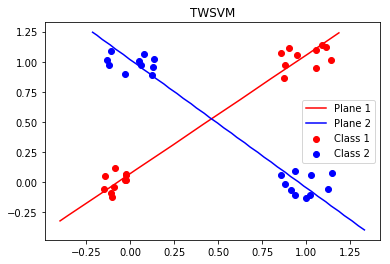
\includegraphics[height=5cm]{./img/TWSVM-img.png}
\caption{TWSVM}
\label{twsvm1}
\end{figure}
